\chapter{Approach}
\label{chapter:approach}


The Procedural Outdoors Scene Generator is a Python framework that enables researchers and procedural 3D modeling artists to create synthetic video data of realistic outdoor scenes. The main purpose is building a systematic way to collaboratively create outdoor scenes and use them in interactive machine learning tasks.


To generate data, the user of the framework chooses a geographical area to be rendered, defines the procedural graphics primitives to be used on the raw geographic data, and implements the logic of the simulation. The procedural graphics primitives can be re-used and shared as individual assets, alongside the Python code that controls the simulation.

% ###############################################################
\section{Design Requirements}
\label{sec:design-requirements}


\begin{description}
    \item[Automates use of GIS data.] Publicly available Geographic Information Systems (GIS) distribute a variety of data, such as satellite imagery, altitude maps, and data on streets, highways, railroads, buildings and urban zoning areas. The framework includes a method to access and combine multiple data sources into a single 3D environment object containing the raw data for generating a scene.
    \item[Capable of procedural 3D modeling.] Specialized 3D artists can create and modify procedurally generated 3D assets, including their textures and shaders, independently of the research team which implements the simulation logic in Python. Procedural 3D modeling can also be used to create variations of existing static 3D objects and their texture and shader information.
    \item[Open.]  The framework must be based on open-source code, and enable the sharing, distribution and modifying of both user code and procedurally generated 3D objects. The framework is based on the Kubric library, which uses the Blender 3D computer graphics software as  the rendering backend. Both these components are free and open-source, which makes it possible to analyze and modify any component, including the rendering engine.
    \item[Portable and Scalable.]  All components of the framework are easily deployable on cloud hardware. Rendering tasks can be parallelized by running multiple instances of the same parameter settings.
    \item[Interactive Rendering.] The framework must support tasks in which the machine learning algorithm needs to effect changes in the scene. An example of this would be an online reinforcement learning model learning to guide a drone over rail tracks: at each frame, the training algorithm decides of a movement, and the simulation must update its scene based on that movement.
\end{description}


\begin{figure}[ht!]
    \centering
    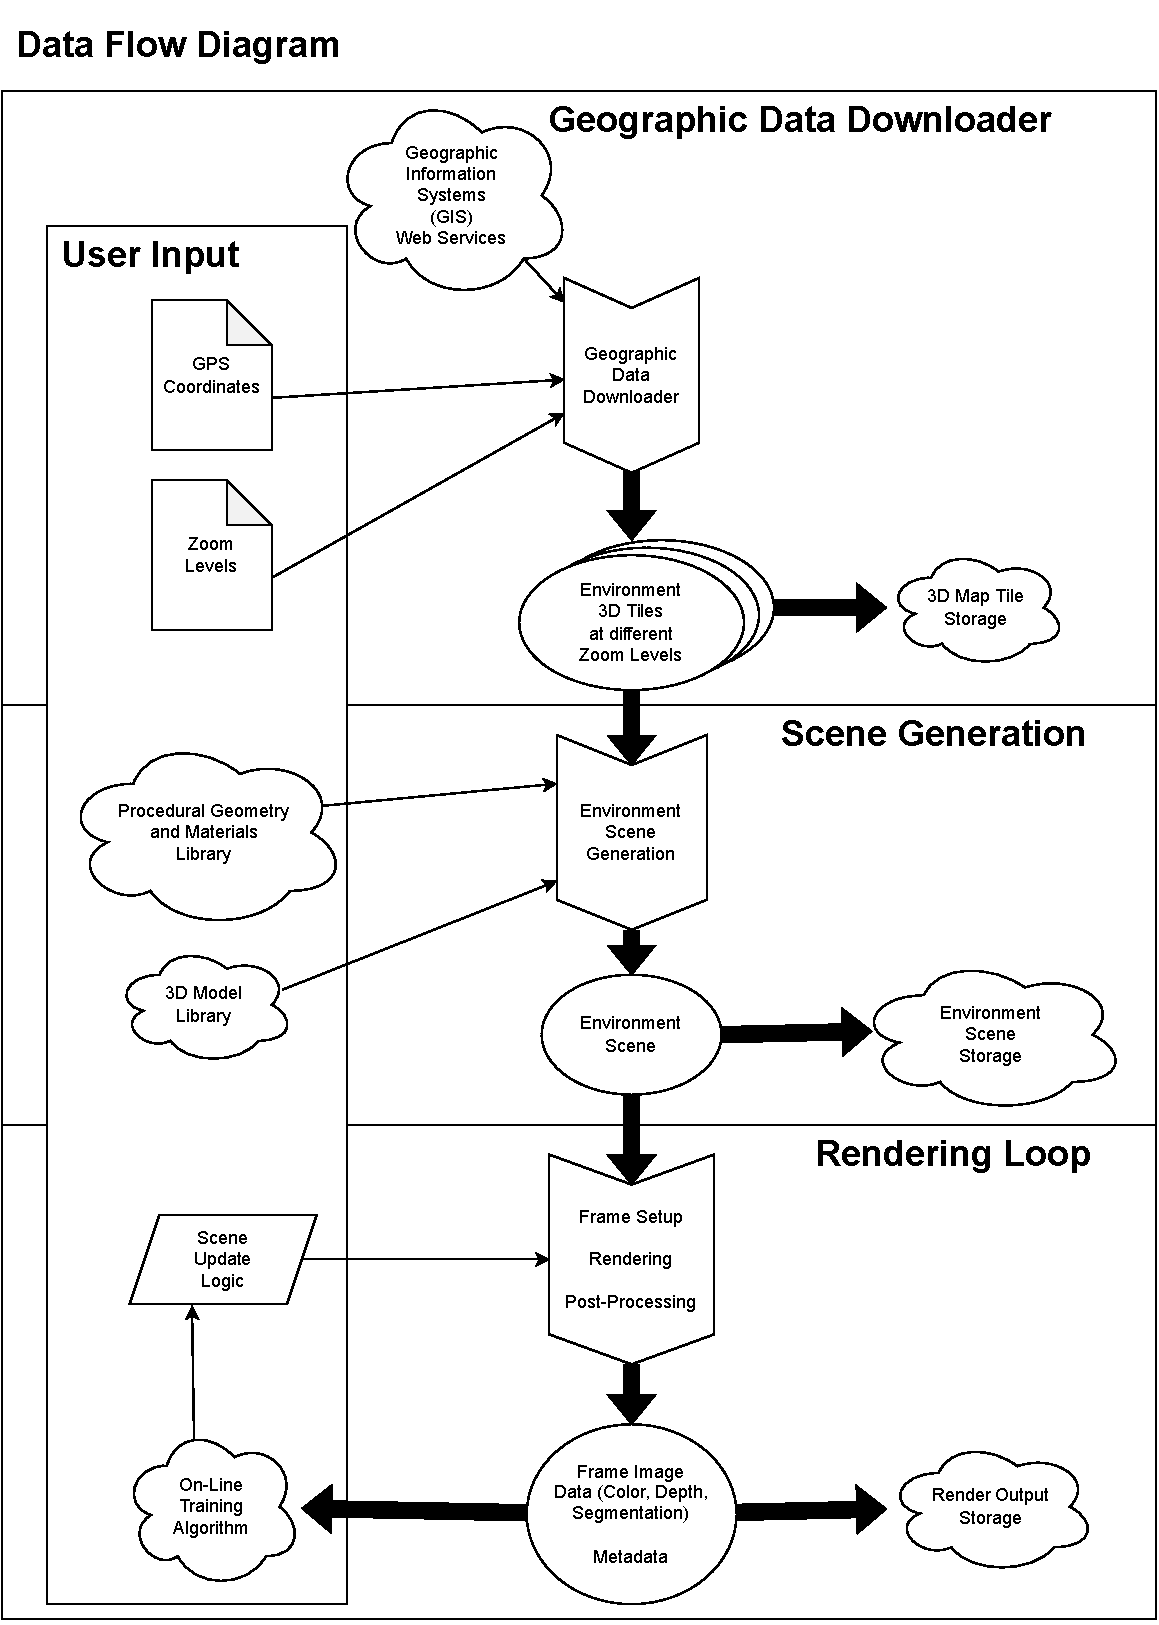
\includegraphics[width=14cm]{src/img/fig/fig-1-overview-v2.drawio-1.pdf}
    \caption{Data Flow Diagram}

    \label{fig:design-overview}
\end{figure}

% ###############################################################
\section{Data Pipeline}
\label{sec:data-pipeline}

The data pipeline contains three main stages: downloading geographic data from various web services; combining it with user-provided procedural geometry, materials and models into a generated 3D environment; and finally using the created environment to render full frames according to user-provided logic that drives the scenarios. This is outlined in the Data Flow Diagram in Figure \ref{fig:design-overview}.



After each of the three stages, the result is saved into a shared storage environment for repeated use in the stages below. For example, the scene generation algorithm can be run with different parameters to rearrange foliage, signage location, and all other randomized environment features, thus leading to more data variation from the same GIS data. In the same way, the render loop can be run multiple times in each scene, while varying the scene parameters for each run.

The design of each stage is discussed in the following sections.

% ###############################################################
\section{Download Stage}
\label{sec:download-stage}

A reproducible process is needed to obtain and combine GIS data from the various providers, including: satellite images from Google Maps and Bing Maps, terrain height maps from Shuttle Radar Topography Mission (SRTM), and road, highway, railway and building data from OpenStreetMap (OSM). The standardization and popularity of these services make it possible to find open-source software components for using them. 

In our case, the Blender GIS plugin is used to combine multiple data sources into a single 3D Scene, containing ground texture and elevation, street and railway paths and building perimeters; see figure \ref{fig:design-data-downloader}. The plugin also supports obtaining a variety of other data types, like urban zoning areas and water bodies.

\begin{figure}[H]
    \centering
    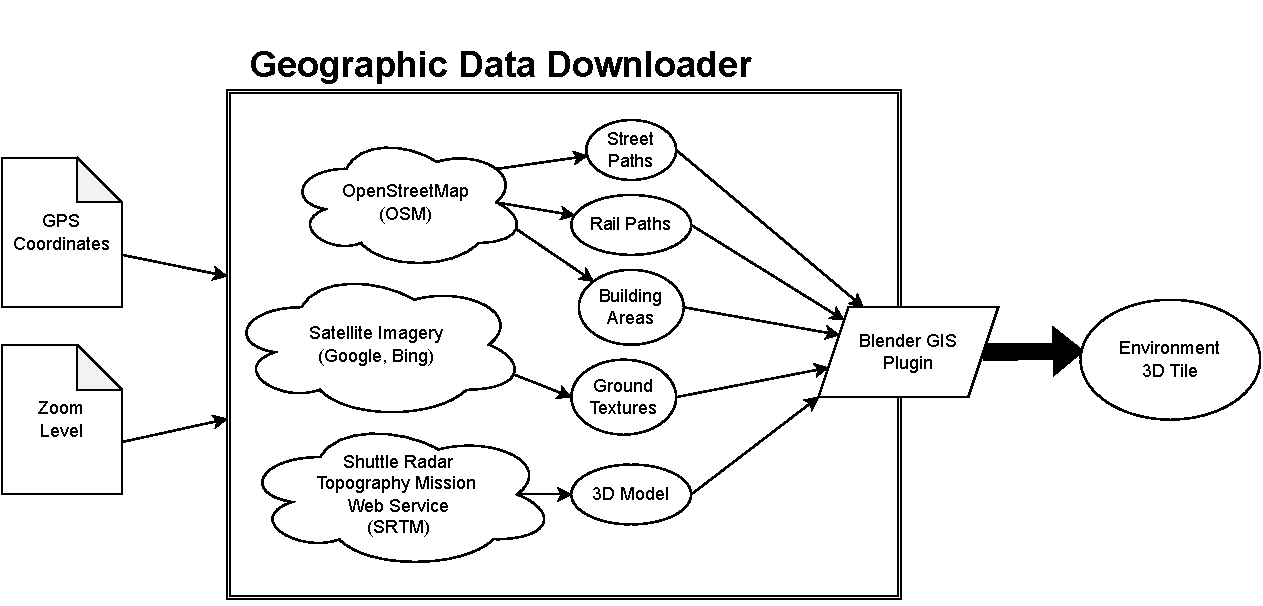
\includegraphics[width=14.5cm]{src/img/fig/fig-2 Geographic Data Downloader.drawio.pdf}
    \caption{Geographic Data Downloader}

    \label{fig:design-data-downloader}
\end{figure}

Each application of the GIS data downloader requires a GPS coordinate and a zoom level, and produces a Blender file containing raw GIS data and metadata, called a 3D tile. For most GIS services, the data resolution is constant, regardless of zoom level. This means we can collect a number of tiles at different zoom levels for the same GPS location, to cover a large geographic area of the background without using a large amount of memory.


% ###############################################################
\section{Procedural Scene Generation Stage}
\label{sec:scene-generation-stage}

This stage collects the 3D tiles stored in the previous step, and combines them into a single terrain object. The data types come from different sources, they are not perfectly aligned with one another. For example, the road and railroad paths from OSM do not perfectly align with the SRTM terrain height maps, or with the Google Satellite ground textures. Because of these slight incompatibilities, this procedure also requires adjusting the terrain profile to be flat around roads, railroads and building foundations.

The parallelograms in Figure \ref{fig:design-scene-generation} represent user-customizable hooks in the framework, here exemplified for a  railway environment generation task. The pipeline results in a single 3D environment scene, containing all static features of the scene, such as railways, roads, signage and electric poles, vegetation and buildings. The result can be stored as a Blender file prior to rendering.

\begin{figure}[H]
    \centering
    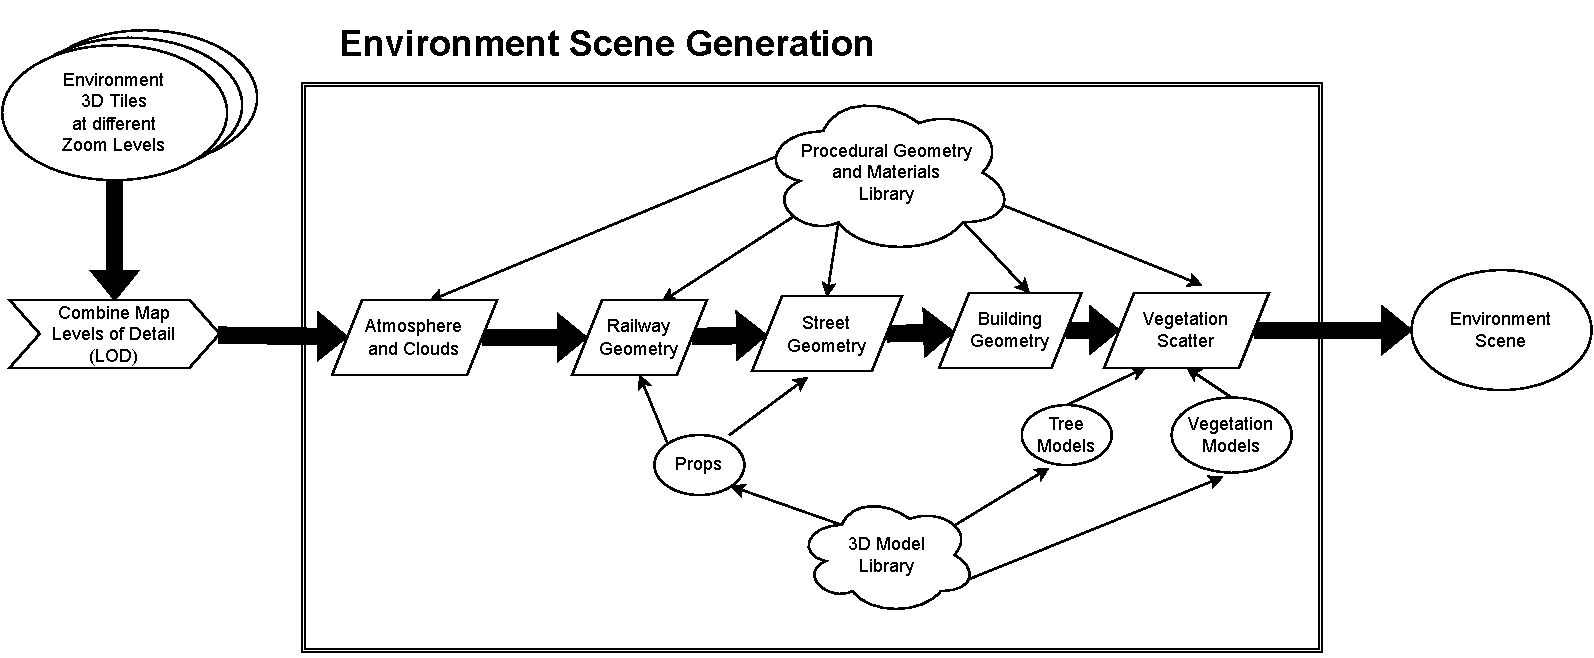
\includegraphics[width=14.5cm]{src/img/fig/fig-3 environment scene generation.drawio.pdf}
    \caption{Scene Generation}
    \label{fig:design-scene-generation}
\end{figure}


% ###############################################################
\section{Render Stage}
\label{sec:render-stage}


The render stage can be used in two ways: with or without externally interacting with a training algorithm.

In the non-interactive case, this stage uses the user-supplied environment scene parameters and frame setup functions to configure each frame for rendering. Dynamic objects, such as obstacles and vehicles, are also added to the scene based on the setup function. The resulting images and metadata are kept in storage, resulting in a dataset that can be used for offline learning. The process is outlined in Figure \ref{fig:design-render-non-interactive}.


\begin{figure}[h]
    \centering
    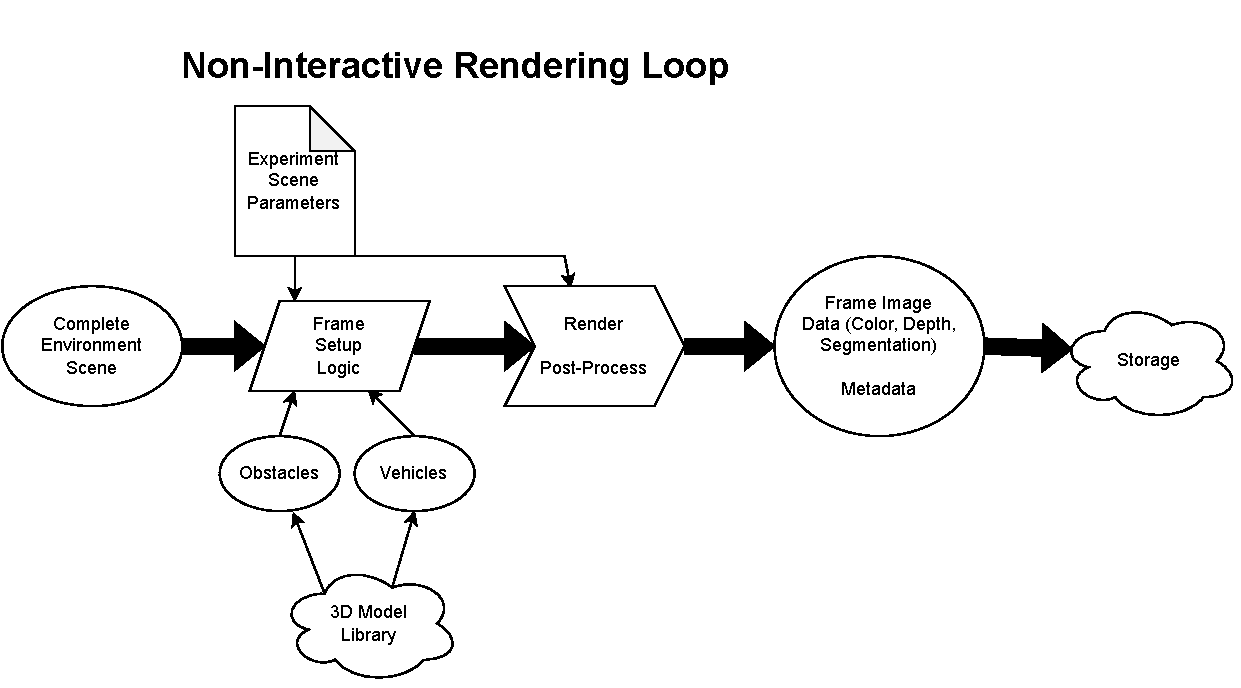
\includegraphics[width=14.5cm]{src/img/fig/fig-4 non-interactive render loop.drawio.pdf}
    \caption{Non-Interactive Render Loop}
    \label{fig:design-render-non-interactive}

\end{figure}


In the case when some online training algorithm is used, the environment is affected by this algorithm at every step. In this case, the render  stage sends its resulting images and metadata to the user-provided training algorithm. The result of this algorithm is used by the user-provided functions to update the scene parameters and then configure the next frame. The rendered images and metadata can optionally be stored for later use; see Figure \ref{fig:design-render-interactive}.

\begin{figure}[h]
    \centering
    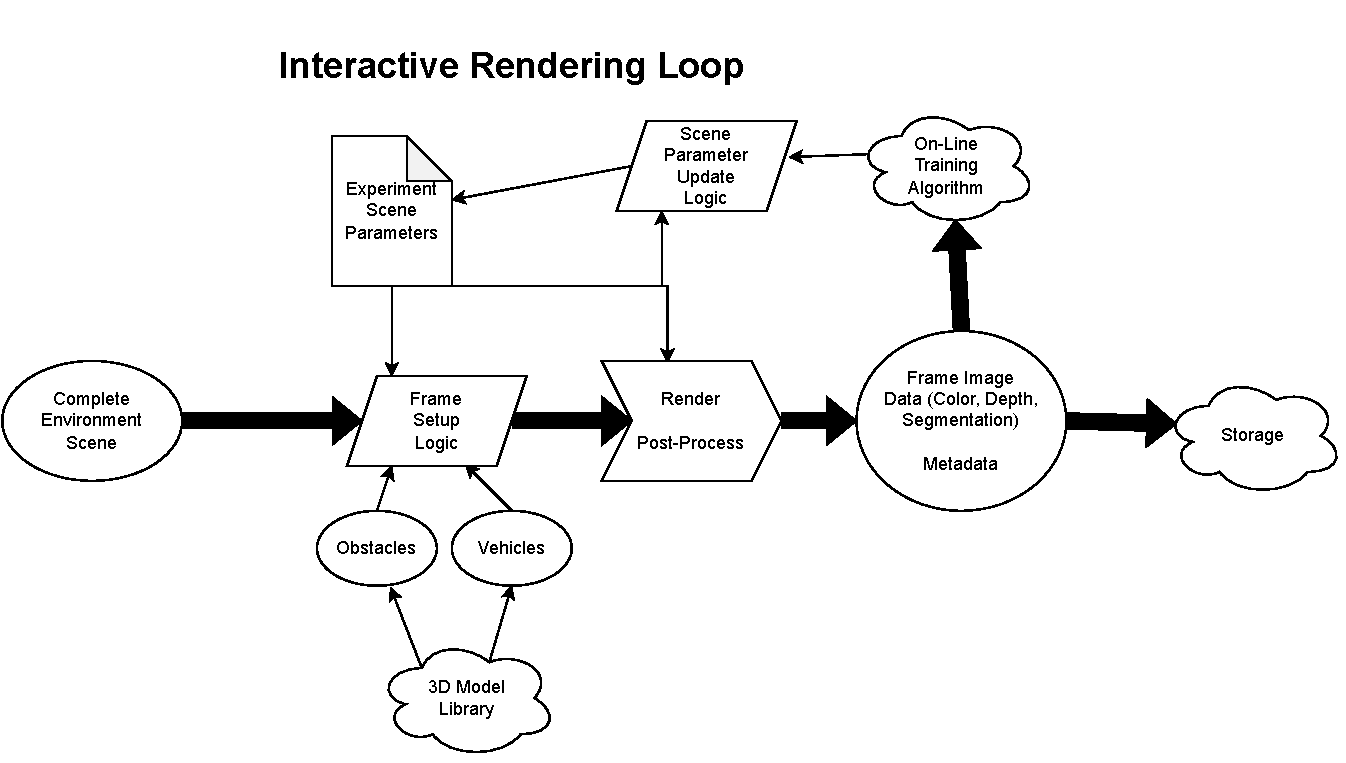
\includegraphics[width=14.5cm]{src/img/fig/fig-5 interactive render loop.drawio.pdf}
    \caption{Interactive Render Loop}
    \label{fig:design-render-interactive}
\end{figure}

The main difference between these two kinds of render loops is how scalability is achieved: in the non-interactive case, each scene frame can be rendered independently, provided the scene logic is deterministic. The interactive case, however, needs to scale the renderers together with the online training algorithm workers, with concurrent rendering of sequential frames not possible.